\documentclass[12pt,english,french]{report}
\usepackage[francais]{babel}
\usepackage[T1]{fontenc}
\usepackage{lmodern}
\usepackage[utf8]{inputenc}
\include{rpu-2012.sty}
\usepackage{numprint}
% la ligne qui suit donne un titre interne au document pdf et crée des liens cliquables en bleu sur les tables et figures
\usepackage[pdftitle={RPU2012-Resural}, colorlinks=true, linkcolor=blue,citecolor=blue, urlcolor=blue, linktocpage=true, breaklinks=true]{hyperref}

\usepackage{makeidx}
\makeindex
\makeglossary

%
% Début du document
% ------------------
%
\usepackage{Sweave}
\begin{document} 
\Sconcordance{concordance:rpu2012.tex:rpu2012.Rnw:%
1 18 1 1 0 12 1 1 12 1 5 69 1 1 4 1 1 1 9 20 0 1 2 6 1 1 8 31 0 1 2 10 %
1 1 4 10 1 1 6 26 1 1 4 7 1 1 8 14 0 1 2 7 1 1 7 14 1 2 2 13 1 1 2 19 0 %
1 1 1 2 3 1}
\Sconcordance{concordance:rpu2012.tex:./rpu2012Latex/rapport/annexes.Rnw:ofs 300:%
1 21 1}
\Sconcordance{concordance:rpu2012.tex:rpu2012.Rnw:ofs 322:%
281 3 1}



\title{Analyse des données RPU 2012 de la région Alsace}
\author{RESURAL}
\date{\today}
\maketitle

\tableofcontents
\listoftables
\listoffigures



%\frontmatter

%\mainmatter

\section{Préambule}

Le présent document est une analyse partielle et incomplète des résumés des passages aux urgences (RPU) produits par une partie des hôpitaux d'Alsace ayant une autorisation de faire fonctionner un service d'urgence au cours de l'année 2012. C'est la première année que cette ébauche d'analyse est faite. En raison du caractère très incomplet des données, il ne peut être
tirés de conclusions définives sur le fonctionnement des urgences. C'est un jeu d'essai qui permet d'apprécier comment les RPU sont compris et saisis, quelles sont les difficultés potentielles sur lesquelles doit porter un effort pédagogique et final permettre d'ébaucher une stratégie d'analyse de ces informations.

\chapter{La région Alsace}
\section{Les secteurs sanitaires}
\section{Les zones de proximité}
\section{Démographie}
Les calculs sont effectués à partir du fichier xxx de l'INSEE qui recense l'ensemble de la population par commune et par tranches de un an. La version utilisée est celle du 1er janvier 2010 (tab.\ref{pop}).

\begin{table}
\begin{center}
\begin{tabular}{|l|l|r|r|}
  \hline
  Tranche d'age & Abréviation & Effectif & Pourcentage \\
  \hline
  \hline
  Moins de 1 an & pop0 & $21903.14$ & 1.19 \\
  De 1 à 75 ans & pop1\_75 & $1690073.00$ & 92.00 \\
  Plus de 75 ans& pop75 & $125110.90$ & 6.81 \\
  \hline
  Total & pop\_tot & $1837087.00$ & 100.00 \\
  \hline
\end{tabular}
\caption{Population d'Alsace (janvier 2010)}
\label{pop}
\end{center}
\end{table}

\section{Les services d'accueil des urgences (SAU)}

\begin{table}
\begin{center}
\begin{tabular}{|c|c|c|c|l|}
  \hline
& Finess utilisé & Finess géographique & Finess Juridique & Structure \\
  \hline
  \hline
1 & 670780055 &   & 670780055 & HUS \\
2 & 670780543 & 670000272 & 670780543 & CH Wissembourg \\
3 & 670000397 & 670000397  & 670780691 & CH Selestat \\
4 & 670780337 & 670000157 & 670780337 & CH Haguenau \\
5 &   & 670000165 & 670780345 & CH Saverne \\
6 & 670016237  & 670016237  & 670016211 & Clinique ste Odile \\
7 &   & 670780212 & 670014604 & Clinique Ste Anne \\
8 & 680000973 & 680000684 & 680000973 & CH Colmar \\
9 & 680000197  & 680000197  & 680000049 & Clinique des trois frontières \\
10 & 680000486 & 680000544  & 680000395 & CH Altkirch \\
11 & 680000700 & 680000700 & 680001005 & CH Guebwiller \\
12 & 680000627 & 680000627 & 680000486 & CH Mulhouse FG \\
13 &   & 680000601 & 680000437 & CH Thann \\
14 &   & 680000320  & 680000643 & Diaconat-Fonderie (St Sauveur) \\
\hline
\end{tabular}
\caption{Service d'accueil des urgences d'Alsace}
\label{summary}
\end{center}
\end{table}

%
% chapitre: les données
% ---------------------
%
\chapter{Les données}

\section{Origine des données}

Les données proviennent des RPU produits par les hôpitaux d'Alsace ayant l'autorisation de faire fonctionner un service d'urgence (SU). La liste des structures hospitalières ayant fournit des informations alimentant le présent rapport est fournie par la table \ref{tab1}, page \pageref{tab1}.

% latex table generated in R 2.15.1 by xtable 1.7-1 package
% Fri Apr 19 16:27:38 2013
\begin{table}[ht]
\centering
\begin{tabular}{|l|r|r|l|r|}
  \hline
 & n & \% & Hôpitaux & Date d'inclusion \\ 
  \hline
Wis & 7711 & 5.42 & CH Wissembourg & 23/04/2012 \\ 
  Sel & 26339 & 18.5 & CH Sélestat & 17/02/2012 \\ 
  Odi & 12354 & 8.68 & Clinique Ste Odile & 30/06/2012 \\ 
  Hus & 35889 & 25.21 & Hôpitaux Universitaires de Strasbourg & 10/02/2012 \\ 
  Hag & 725 & 0.51 & CH Haguenau & 18/06/2012 \\ 
  3Fr & 7342 & 5.16 & Clinique des 3 frontières & 09/07/2012 \\ 
  Alk & 169 & 0.12 & CH Altkirch & 27/11/2012 \\ 
  Col & 46927 & 32.96 & CH Colmar & 01/01/2012 \\ 
  Geb & 4920 & 3.46 & CH Guebwiller & 01/09/2012 \\ 
   \hline
\end{tabular}
\caption{Structures hospitalières participantes en 2012} 
\label{tab1}
\end{table}
\section{Exhaustivité des données}

Les informations de nature administrative (code postal, commune d'origine, sexe, date de naissance,\dots ) sont correctement renseignées avec une exhaustivité de $100\%$.

Les données à caractère plus médical comme le motif de consultation ou le diagnostic principal ont une exhaustivité moins bonne, de l'ordre de $70\%$.

% latex table generated in R 2.15.1 by xtable 1.7-1 package
% Fri Apr 19 16:27:39 2013
\begin{table}[ht]
\centering
\begin{tabular}{|l|r|}
  \hline
 & \% \\ 
  \hline
id & 0.00 \\ 
  CODE\_POSTAL & 0.00 \\ 
  COMMUNE & 0.00 \\ 
  ENTREE & 0.00 \\ 
  EXTRACT & 0.00 \\ 
  FINESS & 0.00 \\ 
  NAISSANCE & 0.00 \\ 
  SEXE & 0.00 \\ 
  AGE & 0.00 \\ 
  MODE\_ENTREE & 3.57 \\ 
  SORTIE & 9.66 \\ 
  GRAVITE & 14.92 \\ 
  MODE\_SORTIE & 15.08 \\ 
  DP & 23.76 \\ 
  TRANSPORT & 27.09 \\ 
  TRANSPORT\_PEC & 29.96 \\ 
  PROVENANCE & 32.75 \\ 
  MOTIF & 34.06 \\ 
  ORIENTATION & 71.36 \\ 
  DESTINATION & 72.51 \\ 
   \hline
\end{tabular}
\caption{Données manquantes en 2012} 
\label{tab2}
\end{table}

Les informations sont résumées dans la table \ref{tab2}, page \pageref{tab2}.

%%%%%%%%%%%%%%%%%%%%%%%%%%%%%%%%%%%%%%%%%%%%%
% Résultats
%%%%%%%%%%%%%%%%%%%%%%%%%%%%%%%%%%%%%%%%%%%%%
\chapter{Analyse des données}

\section{Résultats}

Le fichier comporte \numprint{142376} RPU.

%
% AGE
% ------
%

\subsection{Age\index{Age} des patients}

% age et sexe

\begin{itemize}
  \item Age moyen pour l'ensemble 44.21 ans.
  \item Age moyen pour les hommes 41.72 ans.
  \item Age moyen pour les femmes 46.93 ans. 
\end{itemize}

\begin{table}
\begin{center}
\begin{tabular}{|l|c|c|c|c|}
  \hline
   \emph{Age} & Min & Max & Moyenne & Médiane \\
    \hline
    \hline
    Hommes & $0$ & 105 & $41.72$ & 40 \\
    \hline
    Femmes & 0 & 105 & 46.93 & 45 \\
    \hline
    \emph{total} & 0 & 105 & 44.21 & 42 \\
  \hline
\end{tabular}
\caption{Age de l'ensemble des patients}
\label{summary}
\end{center}
\end{table}

Les caractéristiques de la population sont résumées dans la table \ref{summary}, page \pageref{summary}.



% \subsection{Age des patients}
% <<test, child='knitr-input-child.Rnw'>>=
% @

% tranche d'age selon serveur régional

% latex table generated in R 2.15.1 by xtable 1.7-1 package
% Fri Apr 19 16:27:39 2013
\begin{table}[ht]
\centering
\begin{tabular}{rrr}
  \hline
 & effectif & pourcentage \\ 
  \hline
moins de 1 an & 1736 & 1.22 \\ 
  de 1 à 75 ans & 116932 & 82.13 \\ 
  plus de 75 ans & 23712 & 16.65 \\ 
   \hline
\end{tabular}
\caption{Structure d'age de la population des urgences} 
\label{age:serveur}
\end{table}Le serveur régional recueille l'age des patients selon trois modalités: moins de 1 an, entre 1 et 75 ans et plus de 75 ans. On obtient le tableau \ref{age:serveur}. Si on compare ce tableau à celui otenu sur l'ensemble de la population Alsacienne (voir table \ref{pop} page\pageref{pop}), on constate que la population des urgences est plus agée que la population de référence.

%
% SEXE
%-------
%

\subsection{Sexe\index{sexe} des patients}
Il existe une légère prédominance masculine. Le sex-ratio est de 0.92 %


\begin{tabular}{|l|c|c|c|c|}
  \hline
   \emph{Sexe} & $n$ & $\%$ \\
   \hline
   Hommes & \numprint{74269} & \numprint{52.16} \\
   Femmes & \numprint{68106} & \numprint{47.84}\\
   NP & \numprint{1} & \numprint{0}\\
  \hline
\end{tabular}

\begin{figure}
\begin{center}
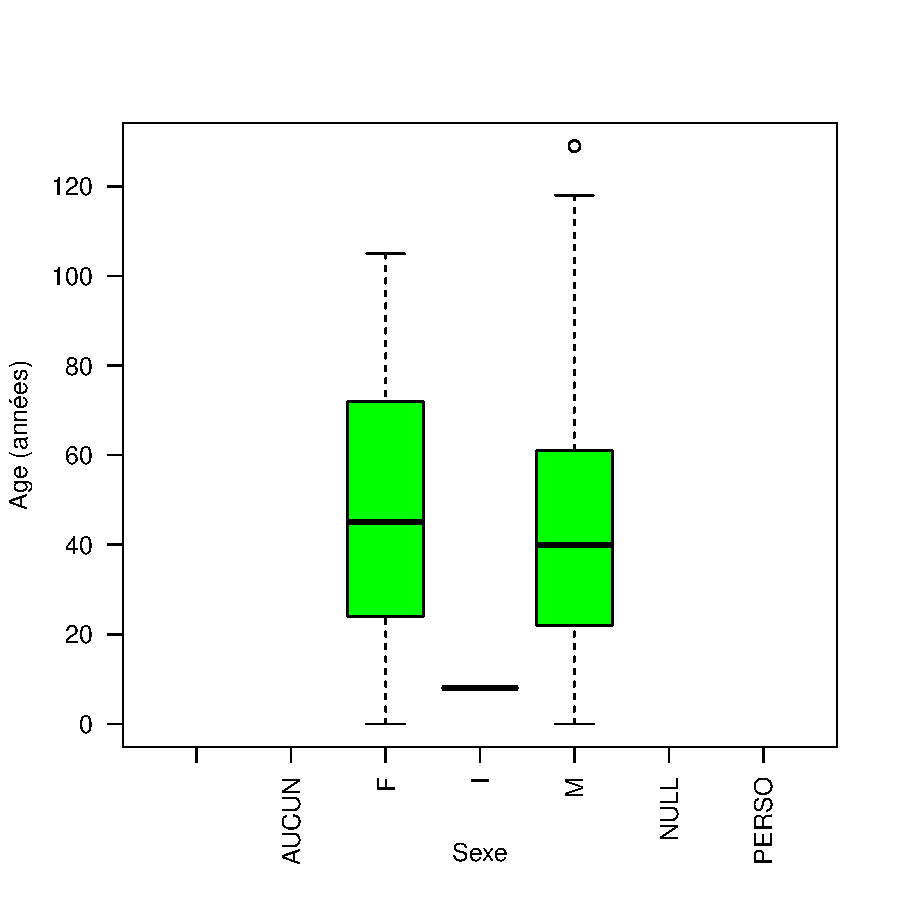
\includegraphics{rpu2012-age_sexe}
\end{center}
\caption{Répartition de l'age en fonction du sexe}
\label{age:sexe}
\end{figure}

L'age moyen des femmes est légèrement plus élevé que celui des hommes (figure \ref{age:sexe} p.\pageref{age:sexe})

%
% Gravité (CCMU)
%----------------
%
\subsection{Gravité (CCMU)\index{gravité} des patients}

La gravité s'évalue à l'aide de la classification clinique des maladies aux urgences (CCMU).
% latex table generated in R 2.15.1 by xtable 1.7-1 package
% Fri Apr 19 16:27:40 2013
\begin{table}[ht]
\centering
\begin{tabular}{rrr}
  \hline
 & n & \% \\ 
  \hline
1 & 21081.00 & 14.80 \\ 
  2 & 82785.00 & 58.10 \\ 
  3 & 13925.00 & 9.80 \\ 
  4 & 1619.00 & 1.10 \\ 
  5 & 390.00 & 0.30 \\ 
  D & 9.00 & 0.00 \\ 
  P & 1325.00 & 0.90 \\ 
  NA & 21242.00 & 14.90 \\ 
   \hline
\end{tabular}
\caption{Répartition de la gravité (CCMU)} 
\label{ccmu}
\end{table}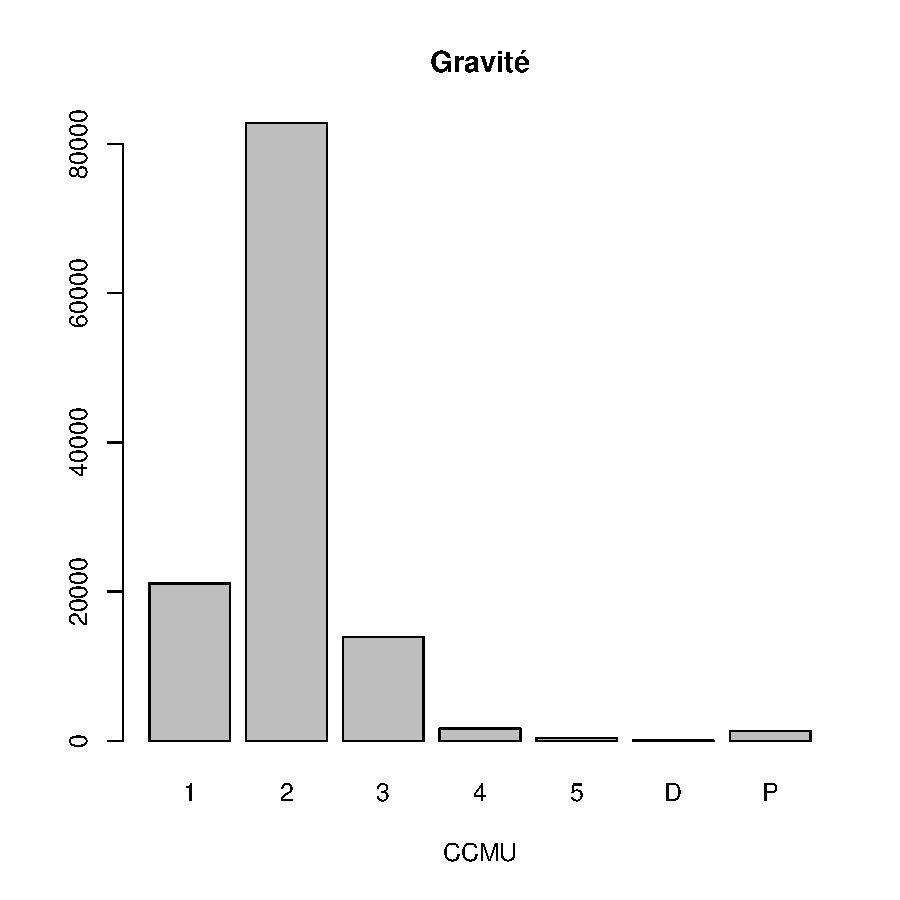
\includegraphics{rpu2012-gravite1}
%%%%%%%%%%%%%%%%%%%%%%%%%%%%%%%%%%%%%%%%%%%%%%%
% A partir de ce point commencent les annexes %
%%%%%%%%%%%%%%%%%%%%%%%%%%%%%%%%%%%%%%%%%%%%%%%
\appendix

\chapter{Résumé de passage aux urgences (RPU)}
La composition d'un RPU répond à une norme définie par l'INVS\footnote{Institut National de Veille Sanitaire} dont la dernière version est datée de 2006. Un RPU se compose des éléments suivants:
\begin{enumerate}
  \item premier
\end{enumerate}

\chapter{Documentation interne}
\begin{enumerate}
  \item Eurostat: Resural\//Stat Resural\//Eurostat\//eurostat\_readme.Rmd
  \item INSEE
  \item Open Street Map (OSM)
  \item cran-R
\end{enumerate}

\section{Logiciel R}
R est un langage de programmation et un environnement mathématique utilisés pour le traitement de données et l'analyse statistique. C'est un projet GNU fondé sur le langage S et sur l'environnement développé dans les laboratoires Bell par John Chambers et ses collègues. 
\
R est un logiciel libre distribué selon les termes de la licence GNU GPL et est disponible sous GNU/Linux, FreeBSD, NetBSD, OpenBSD, Mac OS X et Windows. R s'interface directement avec la pluspart des bases de données courantes: BO (Oracle), MySQL, PostgreeSql, etc. Il s'interface aussi avec un certain nombre de système d'information géographique (SIG) et sait lire nativement le format Shapefile utilisé par l'IGN.
\
Le logiciel R est interfacé avec le traitement de texte Latex par l'intermédiaire de la bibliothèque Sweave. Cette association permet de mélanger du texte et des formules mathématiques produisant les résultats et graphiques de ce document. En cas de modification des données, il suffit de recompiler le fichier source pour mettre à jour le document final.
\

\printindex

\end{document}
